\scanpage{48}
\mspage{\handwritten{16}}
\uline{Alors, pour tout sous-$\handwritten{\mathcal{O}}_S$-Module quasi-cohérent $\handwritten{\mathcal{F}}$ de $\handwritten{\mathcal{E}}$ il existe un plus petit sous-$\handwritten{\mathcal{O}}_S$-Mo-\linebreak dule quasi-cohérent $\handwritten{\widetilde{\mathcal{F}}}$ de $\handwritten{\mathcal{E}}$ contenant $\handwritten{\mathcal{F}}$ qui soit stable sous $\handwritten{\rho}$.}\inserted{\handwritten{Sa formation commute à toute extension de la base $S'\to S$}}\uline{Lorsque $\handwritten{\mathcal{F}}$ est de type \deleted{\unsure{fin}} fini, il en est de même de $\handwritten{\mathcal{F}}$.}

On se ramène aisément\inserted{\handwritten{par descente fidèlement plate}} au cas où $\handwritten{\mathscr{A}}$ est un $\handwritten{\mathcal{O}}_S$-Module libre, auquel cas la proposition est conséquence du lemme 11.8.

\figure{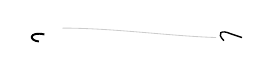
\begin{tikzpicture}[x=1cm,y=1cm]\draw[line width=.7pt] (.12,.04) .. controls (-.08,.08) and (-.08,-.04) .. (.05,-.05);\draw[gray!40,line width=.3pt] (.35,.12) .. controls (1,.12) and (1.7,.02) .. (2.3,0);\draw[line width=.5pt] (2.4,-.04) .. controls (2.3,.06) and (2.37,.1) .. (2.48,.05)--(2.63,0);\end{tikzpicture}}
\uline{Corollaire 11.10.- \deleted{\unsure{Soit}}\inserted{Soient} $S$ un \deleted{pré} schéma \deleted{affine}\inserted{\handwritten{\unsure{quasi-compact|quasicompact} quasi-séparé}}, $G$ un $S$-groupe quasi-séparé\inserted{\handwritten{et}}quasi\unsure{\deleted{\illegible{1}}-|\deleted{\illegible{1}}e}compact sur $S$ , tel que $\handwritten{\mathscr{A}}(G)$ devienne \deleted{\unsure{libre}} localement libre après extension fidèlement plate quasi-com-\linebreak pacte de la base,$S$, et soit $\handwritten{\mathcal{E}}$ un $\handwritten{\mathcal{O}}_S$-Module quasi-cohérent. On suppose soit que $G$ est affine sur $S$\deleted{\unsure{.}}\handwritten{,}soit que $G$ et $\handwritten{\mathcal{E}}$ sont plats sur $S$,\inserted{\uline{On se donne une opération de $G$ sur $\handwritten{\mathcal{E}}$\handwritten{\unsure{;|!}}}} \deleted{\unsure{A|a}}\handwritten{A}lors $\handwritten{\mathcal{E}}$ est limite inductive d'une famille fil-\linebreak trante croissante de sous- $\handwritten{\mathcal{O}}_S$-Modules quasi-cohérents de type fini de $\handwritten{\mathcal{E}}$ stables sous} $\handwritten{G}$.

C'est une conséquence immédiate de (11.9) car $\handwritten{\mathcal{E}}$ est \deleted{engendré par ses sections (EGA I 1.4.1\unsure{)} et car l'ensemble des sous-$\handwritten{\mathcal{O}}_S$-Modules quasi-cohérents de type fini de $\handwritten{\mathcal{E}}$ stables sous $G$ est stable par engendrement.}\inserted{\handwritten{limite inductive de ses sous-Modules quasi-cohérents de type fini (EGA I \unsure{9|1}.4.9. , $\overline{\underline{\mathrm{IV}}}$ 1.7.7.)}}

\uline{Remarque} 11.10.1. J.P. Serre a remarqué que dans 11.9. (donc aussi dans 11.10) il suffisait de supposer que pour toute ouvert affine $U$ de $S$\unsure{;|,} il existe un morphisme fidè\deleted{b}lement plat $U'\handwritten{\to}U$, avec $U'$ affine d'anneau $A'$, tel que $\handwritten{\mathcal{E}\otimes}_U U'$ soit défini par un $A'$-module projectif (pas nécessairement libre). De plus, lorsque $S$ est localement noéthérien régulier et de dimension 1, cette hypothèse peut être remplacée par la seule hypothèse que $G$ soit plat sur $S$ (ce qui implique que $\handwritten{\mathscr{A}}(G)$ est plat); voir à ce sujet \deleted{un exposé de Serre dans SGA}\inserted{\handwritten{6}}\deleted{(1966/67).}\handwritten{1} \inserted{\handwritten{J.P. Serre, \unsure{Sur} le Groupes de Grothendieck des schémas en groupes réductifs déployés, Pub. Math. n° 39, p. 37-52.}}

\deleted{\uline{Proposition 11.11.- Soient $k$ un corps, $G$ un \deleted{corps} $k$-groupe algébrique. Pour que $G$ soit affine, il faut et il suffit qu'il existe un espace vectoriel de dimension finie $V$, et une immersion fermée de $G$ dans $\underline{\mathrm{GL}}_k(V)$ qui soit un morphisme de $k$-groupes.}}

\deleted{S'il existe un espace vectoriel $V$ de dimension finie et une immersion fer\`{m}ée $u:G\handwritten{\to}\underline{\mathrm{GL}}_k(V)$, puisque $\underline{\mathrm{GL}}_k(V)$ est affine (E\deleted{xp}\inserted{XP}. I, 4.5), il en est de même de $G$ (EGA I 4.2.3).}

\deleted{Réciproquement, supposons $G$ affine. Notons $A$ l'algèbre de $G$. Puisque $G$ opère sur lui-mê-\linebreak me par translations à gauche, il op\v{e}re aussi sur $A$, cette opération se traduisant par l'appli-\linebreak cation \deleted{\unsure{diagona|diagonà|diagonal}} diagonale $\handwritten{\Delta}:A\handwritten{\longrightarrow}A\handwritten{\otimes}_k A$. D'après (11.1\handwritten{0}), $A$ (en tant qu'espace vectoriel) est réunion d'une famille filtrante croissante $(V_i)_{i\handwritten{\in}I}$ de sous-espaces vectoriels de dimension fi-\linebreak nie stables sous $G$.}
\deleted{\illegible{1} $\unsure{G}$ \illegible{2} \unsure{type fini sur} $k$, $A$ \illegible{2} \unsure{type fini sur} $k$, \unsure{donc} il \illegible{1} $i_{\unsure{o|0}}\handwritten{\unsure{\in}}I$ tel que $V_{i_{\unsure{o|0}}}$ \unsure{engendre} $\unsure{A}$ \unsure{comme algèbre.} L'\unsure{opération} \illegible{1} $\unsure{G}$ \unsure{sur}}
% archive sheet number: 47
